\section{Theorie}
\label{sec:Theorie}
  \subsection{Prinzip einer Wärmepumpe und ihre Güteziffer}
  Nach dem zweiten Hauptsatz der Themodynamik, der besagt, dass die Entropie in
  einem abgeschlossenen System niemals abnehmen kann, verläuft ein Wärmeaustausch
  zwischen zwei Reservoiren unterschiedlicher Temperatur von selbst immer vom
  Wärmeren zum Kälteren hin.
  Es ist jedoch möglich die Richtung des Wärmetransports umzukehren, wenn dem
  System Energie in Form von mechanischer Arbeit zuführt wird. Ist dies der Fall,
  so spricht man von einer Wärmepumpe.

  Aus dem Verhältnis der aufzuwendenden Arbeit A und der an das wärmere Reservoir
  abgegebenen Wärmemenge $Q_1$ resultiert die Güteziffer $v$ einer Wärmepumpe.
  Da nach dem ersten Hauptsatz der Themodynamik die totale Energie ein einem
  abgeschlossenen System erhalten bleiben muss, muss die abgegebene Wärmemenge
  $Q_1$ gleich der Summe aus der aufgewandten Arbeit und der aus dem kälteren
  Reservoir entnommenen Wärmemenge $Q_2$ sein:
  \begin{equation}
    Q_1 = Q_2 + A
    \label{eqn:gl1}
  \end{equation}
  Damit ist
  \begin{equation}
    v = \frac{Q_1}{A}
    \label{eqn:gueteziffer1}
  \end{equation}
  der Wirkungsgrad einer Wärmepumpe.

  Unter der Voraussetzung, dass sich die Temperaturen in den Reservoiren während
  der Wärmeübertragung nicht ändern und der Prozess reversibel verläuft, folgt
  aus dem zweiten Hauptsatz der Themodynamik, dass die Summe der reduzierten
  Wärmemengen $\int \! \frac{\symup{d}Q}{T}$ verschwindet:
  \begin{equation}
    \frac{Q_1}{T_1} - \frac{Q_2}{T_2} = 0
    \label{eqn:gl3}
  \end{equation}
  Reversibilität bedeutet in diesem Zusammenhang, dass der Prozess des
  Energieaustausches zu jedem Zeitpunkt verlustfrei umgekehrt werden kann.
  Dies ist jedoch nur bei idealen Systemen gegeben, so dass für den irreversiblen,
  realen Fall nur die Ungleichung
  \begin{equation}
    \frac{Q_1}{T_1} - \frac{Q_2}{T_2} > 0
    \label{eqn:gl4}
  \end{equation}
  gilt.

  Verwendet man Gleichung \eqref{eqn:gl3} in \eqref{eqn:gl1}, so ergibt sich nach
  \eqref{eqn:gueteziffer1} die Güteziffer für eine ideale Wärmepumpe:
  \begin{equation}
    v_\symup{ideal} = \frac {Q_1}{A} = \frac{T_1}{T_1 - T_2}.
    \label{eqn:gueteziffer_ideal}
  \end{equation}
  Analog gilt mit \eqref{eqn:gl1} und \eqref{eqn:gl4} nach Gleichung \eqref{eqn:gueteziffer1}
  für die reale Wärmepumpe
  \begin{equation}
    v_\symup{real} < \frac{T_1}{T_1 - T_2}.
    \label{eqn:gueteziffer_real}
  \end{equation}
  Daraus kann man leicht erkennen, dass die Wärmepumpe einen besseren Wirkungsgrad
  hat, je geringer die Temperaturdifferenz zwischen den Reservoiren ist.



  \subsection{Aufbau und Funktionsweise einer Wärmepumpe}
  \begin{figure}
    \centering
    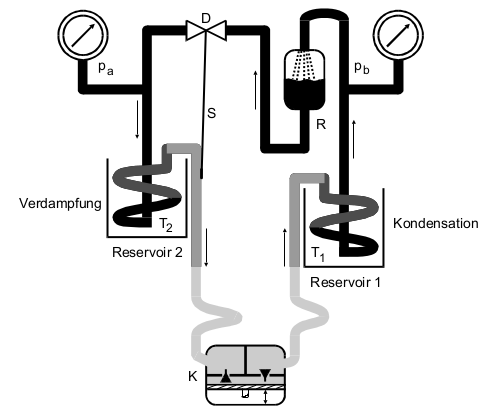
\includegraphics[width=0.65\textwidth]{aufbau_waermepumpe.png}
    \caption{Aufbau einer Wärmepumpe\cite{sample}.}
    \label{fig:aufbau}
  \end{figure}
  In Abbildung \ref{fig:aufbau} ist der schematische Aufbau einer Wärmepumpe zu
  sehen. Wichtige Elemente sind die Reservoire 1 und 2, welche mit einer genau
  definierten Menge Wasser gefüllt sind, und in denen sich Kupferspiralen für den
  Wärmeaustausch zwischen Transportmedium und Wasser befinden. Bei dem Transportmedium
  handelt es sich um ein reales Gas, welches eine möglichst hohe Kondensationswärme
  besitzt. In unserem Fall wurde Dichlordiflourmethan ($\ce{Cl2F2C}$) verwendet.
  Das Gas ist bei Temperatur $T_1$ und dem Druck $p_\symup{b}$ flüssig und bei
  $T_2$ und Druck $p_\symup{a}$ gasförmig. Das flüssige Gas verdampft in Reservoir
  2 und entzieht diesem die Verdampfungswärme L. Infolgedessen sinkt die
  Temperatur $T_2$ in Reservoir 2.
  Der Kompressor K komprimiert das Gas, wodurch der Druck $p_\symup{b}$ steigt,
  so dass das Gas in Reservoir 1 kondensiert und dabei die zuvor aufgenommene
  Verdampfungswärme als Kondensationswärme L abgibt. Dadurch steigt die
  Temperatur $T_1$ in Reservoir 1.
  Zwischen den Reservoiren liegt das Drosselventil D, welches durch Strömungswiderstände
  den Druckunterschied zwischen $p_\symup{b}$ und $p_\symup{a}$ erzeugt.
  Der Reiniger R und die Steuerungsvorrichtung S gewährleisten eine störungsfreien
  Funktionsweise. Der Reiniger entfernt verbliebene Gasreste aus dem flüssigen
  Medium, die Steuerungsvorrichtung regelt den Durchlass des Drosselventils.


  \subsection{Kenngrößen einer Wärmepumpe}
  Zur Beurteilung einer Wärmepumpe ist ihre Güteziffer $v$, der Massendurchsatz
  $\frac{\symup{d}m}{\symup{d}t}$ des Transportmediums und der Wirkungsgrad des
  Kompressors von Interesse. Wie diese Kenngrößen aus den Messwerten bestimmt werden
  können wird nachfolgend beschrieben.
  \subsubsection{Bestimmung der realen Güteziffer $v_\symup{real}$}
  Aus den gemessenen Temperaturen $T_1$ pro Zeitintervall $\Delta t$ wird die pro
  Zeitintervall gewonnene Wärmemenge
  \begin{equation}
    \frac{\Delta Q_1}{\Delta t} = (m_1 c_w + m_k c_k) \frac{\Delta T_1}{\Delta t}
    \label{eqn:waermeprozeit1}
  \end{equation}
  berechnet. Dabei ist $m_1 c_w$ die Wärmekapazität des Wassers in Reservoir 1
  und $m_k c_k$ die Wärmekapazität der Kupferschlange und des Behälters gemeinsam.
  Mit der über $\Delta t$ gemittelten Leistungsaufnahme des Kompressors N ergibt
  sich für die Güteziffer mit \eqref{eqn:waermeprozeit1}
  \begin{equation}
    v_\symup{real} = \frac{\Delta Q_1}{N\Delta t} = \frac{m_1 c_w + m_k c_k}{N} \frac{\Delta T_1}{\Delta t}.
    \label{eqn:berechnung_gueteziffer}
  \end{equation}


  \subsubsection{Bestimmung des Massendurchsatzes}
  Gleichung \eqref{eqn:waermeprozeit1} lässt sich analog für Reservoir 2 für
  $\Delta T_2$ aufstellen:
  \begin{equation}
    \frac{\Delta Q_2}{\Delta t} = (m_2 c_w + m_k c_k) \frac{\Delta T_2}{\Delta t}.
    \label{eqn:waermeprozeit2}
  \end{equation}
  Die Wärmeentnahme geschieht in Form der Verdampfungswärme $L$ pro Massen- und
  Zeiteinheit. Der Massendurchsatz lässt sich mit \eqref{eqn:waermeprozeit2} berechnen,
  wenn $L$ bekannt ist:
  \begin{equation}
    \frac{\Delta m}{\Delta t} = \frac{\Delta Q_2}{L\Delta t}
    = \frac{m_2 c_w + m_k c_k}{L} \frac{\Delta T_2}{\Delta t}
    \label{eqn:massendurchsatz}
  \end{equation}


  \subsubsection{Bestimmung der mechanischen Kompressorleistung $N_\symup{mech}$}
  Die Arbeit $A_\symup{mech}$, die von dem Kompressor verrichtet wird, wenn er ein
  Gasvolumen $V_\symup{a}$ auf das Volumen $V_\symup{b}$ verdichtet, ist
  \begin{equation}
    A_\symup{mech} = - \int_{V_\symup{a}}^{V_\symup{b}} \!p \,\symup{d}V
    \label{eqn:arbeit_kompressor}
  \end{equation}
  Unter der idealisierten Annahme, dass die Kompression des Gases adiabatisch erfolgt,
  gilt die Poissonsche Gleichung
  \begin{equation}
    p_\symup{a} V_\symup{a}^\kappa = p_\symup{b} V_\symup{b}^\kappa = p V^\kappa
    \label{eqn:poissongl}
  \end{equation}
  mit $\kappa = \frac{C_\symup{p}}{C_\symup{v}}$, $\kappa > 1$ und den Molwärmen
  $C_\symup{p}$ (für konstanten Druck) und $C_\symup{V}$ (für konstantes Volumen).
  Dies wird nach $p$ umgeformt und in Gleichung \eqref{eqn:arbeit_kompressor}
  eingesetzt. Für $A_\symup{mech}$ ergibt sich dann
  \begin{equation}
    A_\symup{mech} = - p_\symup{a} V_\symup{a}^\kappa
    \int_{V_\symup{a}}^{V_\symup{b}} V^{-\kappa} \symup{d}V
    = \frac{1}{\kappa - 1}\left(p_\symup{b} \sqrt[\kappa]{\frac{p_\symup{a}}{p_\symup{b}}}
    - p_\symup{a} \right) V_\symup{a}
    \label{eqn:arbeit2}
  \end{equation}
  und für die mechanische Kompressorleistung
 \begin{equation}
   N_\symup{mech} = \frac{\Delta A_\symup{mech}}{\Delta t}
   = \frac {1}{\kappa - 1}\left(p_\symup{b} \sqrt[\kappa]{\frac{p_\symup{a}}{p_\symup{b}}}
   - p_\symup{a} \right) \frac{1}{\rho} \frac{\Delta m}{\Delta t}
   \label{eqn:kompressorleistung}
 \end{equation}
 $\rho$ ist dabei die Dichte des Gases bei dem Druck $p_\symup{a}$. Die Bestimmung
 von $\rho$ ist über die Ideale Gasgleichung $pV=Nk_\symup{b}T$ und $\rho_0$, also
 der Dichte bei Normalbedingungen möglich.
\cite{sample}
